\section{First Trajectory}
Firstly the initial and final values of of $\theta$ and $\dot{\theta}$ are known. Further, the $\theta$-dynamics are known, also for non-zero forces. In the state space and general equations, \autoref{eq:stateSpaceThetaDynamics} and \autoref{eq:alphaBetaGammaGeneral}, the input force is contained by the $\gamma$-function.\\
If now \autoref{eq:alphaBetaGammaGeneral} is seen as an initial value problem. After some manipulation, \fxnote{source Anton's paper(s)} \fxnote{maybe include further explanation/derivations} it is seen that the following function preserves its zero value along the trajectory from initial to final value, assuming the solution exists while requiring $\alpha$ to be non-zero,
%
\begin{flalign}
  \dot{\theta}^2 - \psi (\theta_0, \theta)
  \left(
  \dot{\theta}_0^2 - \int\limits_{\theta_0}^{\theta} \psi (\theta_0, \theta)
  \frac{2 \gamma(s) }{ \alpha(s) } ds
  \right)
  &=  0   \ \ \ , & %\unit{N \cdot m}
  \label{eq:ipv}
\end{flalign}
\ \ \  where,
\begin{flalign}
  \ \ \ \ \ \ \ \psi (\theta_0, \theta) &=
  \exp \left\{
         -2 \int\limits_{\theta_0}^{\theta} \frac{\beta(\tau)}{\alpha(\tau)}  d\tau
       \right\}   \ \ \ . \nonumber &
\end{flalign}

It turns out, that in this case the problem can be solved analytically, and by requiring the final value of the angular velocity be zero, it boils down to,
%
\begin{flalign}
  \left[ -f \frac{m l}{M + m} \sin(s) - m g l \cos(s) \right ]_{\theta_0}^\theta &=  0   \ \ \ . & %\unit{N \cdot m}
  \label{eq:solution}
\end{flalign}

Inserting initial and final value of $\theta$ and solving for f, the force which creates the desired trajectory is obtained. Also note that for this trajectory the applied force is constant and negative, pulling the cart to the left.

Going back to the $\theta$-dynamics, it is possible to construct a phase portrait, see \autoref{fig:phasePortraitFirstTrajectry}, including this negative constant force.

\begin{figure}[H]
  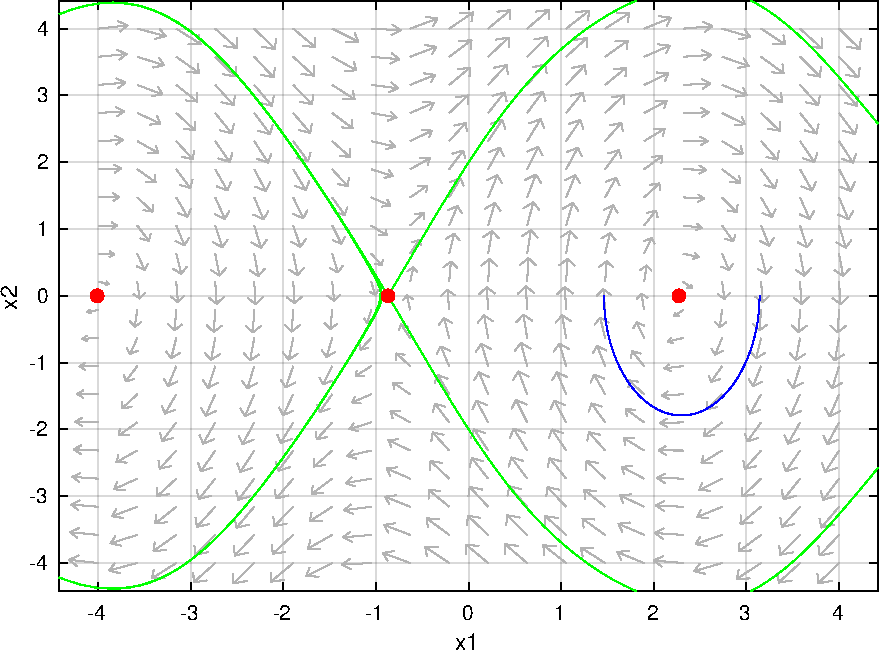
\includegraphics[width=.8\textwidth]{figures/firstTrajectory}
  \caption{Phase portrait of the $\theta$-dynamics including a constant applied force, where $x_1 = \theta$ and $x_2 = \dot{\theta}$. The phase portrait is shifted negatively along $\theta$ because of the applied force. This allows the desired trajectory (blue) from the initial downward position.}
  \label{fig:phasePortraitFirstTrajectry}
\end{figure}

Note how the entire phase portrait is shifted in the negative $\theta$ ($x_1$) direction. This could be expected from \autoref{eq:alphaBetaGamma}, since the force only scales the magnitude of a term which otherwise only depends on $\theta$. Further, the constant force applied is negative, thus the negative shift in the $\theta$ direction.\\
This shift of the phase portrait means that the initial downward position of the pendulum now is placed in an orbit rather than an equilibrium.\\
Additionally, the trajectory (blue) reaches zero angular velocity just as it hits the target angle. The trajectory does however not stop there. It oscillates around the new center equilibrium. Therefore the next input force for the next trajectory must be applied the moment zero angular velocity is achieved.